\documentclass[UTF8,12pt]{ctexart}
%加载包
\usepackage{ctex}
\usepackage{geometry}%排版
%a4版面,页边距1英寸,showframe 增加边框的参数。
% 设置为A4纸,边距适中模式(永中office)
\geometry{%
	width = 210mm,%
	height = 297mm,
	left = 21.8mm,%
	right = 21.8mm,%
	top = 25.4mm,%
	bottom = 25.4mm%
}

%\hyphenpenalty = 1000% 断字设置,值越大,断字越少。
%\setlength{\parindent}{2em}% 缩进
%\setlength{\parskip}{0.5ex} % 段间距

\usepackage{cite} %引用
\usepackage{amsmath}
\usepackage{amsfonts}
\usepackage{amssymb}%公式
\usepackage{amsthm}%定理环境

%\usepackage{ntheorem}%定理环境,使用这个会使\maketitle版式出问题
\usepackage{bm}%加粗

\usepackage{mathrsfs}
\numberwithin{equation}{section}%对公式以节{section}为基础进行编号.变成(1.1.1)有chapter才有1.1.1,不然只有section是1.1
%\theoremstyle{plain}%定理用latex默认的版式
\newtheorem{thm}{Theorem}[section]
%\theoremstyle{definition}%定义用definition格式
\newtheorem{defn}{Definition}
%\theoremstyle{remark}%用remark格式
\newtheorem{lemma}[thm]{lemma}
\newtheorem{example}{Example}[section]

\usepackage{multirow}%表格列合并宏包,\multirow命令.

\usepackage{tabularx}%表格等宽,\begin{tabularx}命令.

 
%盒子
\usepackage{mdframed} % 用于创建盒子
\usepackage[many]{tcolorbox}    	% for COLORED BOXES (tikz and xcolor included)
\usepackage{setspace}               % for LINE SPACING
\usepackage{multicol}               % for MULTICOLUMNS
%自定义设定		
	\definecolor{main}{HTML}{5989cf}    % setting main color to be used
	\definecolor{sub}{HTML}{cde4ff}     % setting sub color to be used
	
	\newtcolorbox{boxF}{
		colback=blue!5!white,
		enhanced,
		boxrule = 1.5pt, 
		colframe = white, % making the base for dash line
		borderline = {1.5pt}{0pt}{main, dashed} % add "dashed" for dashed line
	}
\tcbuselibrary{skins, breakable}% 支持文本框跨页

\usepackage[english]{babel}% 载入美式英语断字模板

\usepackage{graphicx}
\usepackage{float}
\usepackage{subfigure} %插入多图时用子图显示的宏包

%\usepackage{algorithm,algorithmic}%算法
\usepackage{algorithm}
%\usepackage{algorithmic}
\usepackage{algpseudocode}

\usepackage{listings}   %代码块
\usepackage{xcolor}
\definecolor{codegreen}{rgb}{0,0.6,0}
\definecolor{codegray}{rgb}{0.5,0.5,0.5}
\definecolor{codepurple}{rgb}{0.58,0,0.82}
\definecolor{backcolour}{rgb}{0.95,0.95,0.92}
%设置代码块
\lstdefinestyle{mystyle}{
	backgroundcolor=\color{backcolour},   
	commentstyle=\color{codegreen},
	keywordstyle=\color{magenta},
	numberstyle=\tiny\color{codegray},
	stringstyle=\color{codepurple},
	basicstyle=\ttfamily\footnotesize,
	breakatwhitespace=false,         
	breaklines=true,                 
	captionpos=b,                    
	keepspaces=true,                 
	numbers=left,                    
	numbersep=5pt,                  
	showspaces=false,                
	showstringspaces=false,
	showtabs=false,                  
	tabsize=2
}

\lstset{style=mystyle,
	language=R,                                       % 设置语言
}

\usepackage{appendix}%附录

\usepackage{hyperref}%可以生成pdf书签,可以跳转
\hypersetup{
	colorlinks=true,
	linkcolor=black,
	citecolor=black,
}%使得目录没有红框 参考文献引用没有颜色

%侧栏笔记
\usepackage{marginnote}
\setlength{\marginparwidth}{2.8cm}%设置宽度
\renewcommand*{\marginfont}{\color{violet}\footnotesize}%fonts
%运用此命令就可加入侧栏笔记\normalmarginpar\marginnote{}




%图注
\usepackage{caption}

%参考文献
\usepackage[round]{natbib}


%画图
\usepackage{tikz}
\usetikzlibrary{matrix,shapes, backgrounds}
\newcommand{\customrule}{%
	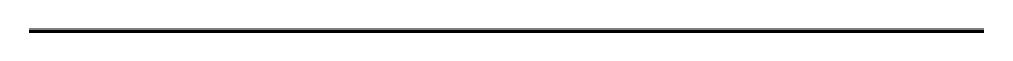
\begin{tikzpicture}
		\draw[gray, thick] (0,0) -- (\linewidth,0);
		\draw[black, thick] (0,-1pt) -- (\linewidth,-1pt);
	\end{tikzpicture}
}

\newcommand{\highlightbox}[1]{%
	\tikz[baseline=(X.base)] 
	\node [draw, thick, rectangle, fill=gray!20, inner sep=2mm] (X) {#1};%
}

%标题页
\title{HMM}
\author{Renhe W.}
\date{ }

%工具
%使用文本框
%\begin{tcolorbox}[enhanced]	\end{tcolorbox}
%代码框
%{\setmainfont{Courier New Bold}                       %设置代码字体                   
%\begin{lstlisting}

%\end{lstlisting}}

%文章开始部分

\begin{document}
	\captionsetup[figure]{labelfont={bf},labelformat={default},labelsep=period,name={图}}%设置图注
	
	\maketitle
	\tableofcontents%目录
	\listoffigures%图片目录
	\listoftables%表格目录
	\newpage
	\kaishu
	
	
	%------------------------------------------- 
	\section{隐马尔可夫模型}
	隐马尔可夫模型 (Hidden Markov Model, HMM)是一个统计模型,用于描述一个隐藏的马尔可夫链产生的观测序列. 系统被假定为一个马尔可夫过程(即无记忆的随机过程)与不可观察(隐藏)的状态.
	
	HMM有两个序列:一个是观测序列,另一个是隐藏的状态序列. 具体形式如图\ref{fig:HiddenMarkov}:
	\begin{figure}[H]
		\centering
		\resizebox{5in}{!}{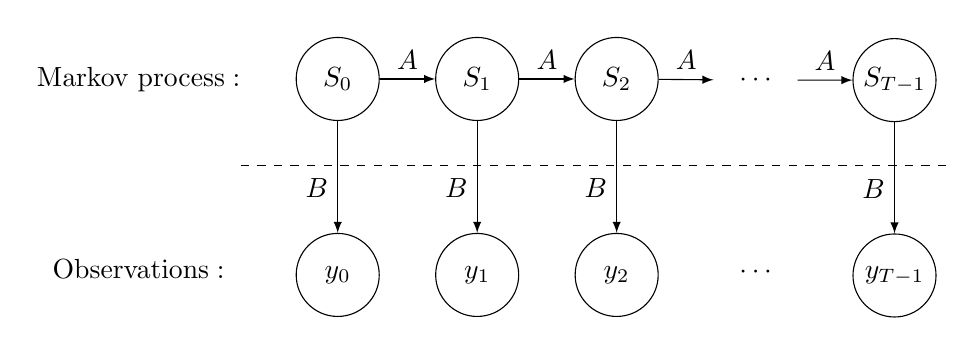
\begin{tikzpicture}
				\matrix[matrix of math nodes,column sep=2em,row
				sep=4em,cells={nodes={circle,draw,minimum width=3em,inner sep=0pt}},
				column 1/.style={nodes={rectangle,draw=none}},
				column 5/.style={nodes={rectangle,draw=none}},
				ampersand replacement=\&] (m) {
					\text{Markov process}: \&
					S_0 \& S_1 \& S_2 \& \cdots \& S_{T-1}\\
					\text{Observations}: \& 
					y_0 \& y_1 \& y_2 \& \cdots \& y_{T-1}\\
				};
				\foreach \X in {2,3,4,5}
				{\draw[-latex] (m-1-\X) -- (m-1-\the\numexpr\X+1) node[midway,above]{$A$};
					\ifnum\X=5
					\draw[-latex] (m-1-6) -- (m-2-6) node[pos=0.6,left]{$B$};
					\else
					\draw[-latex] (m-1-\X) -- (m-2-\X) node[pos=0.6,left]{$B$};
					\fi}
				\draw[dashed] ([yshift=1ex]m.east) -- ([yshift=1ex]m.east-|m-1-1.east);
		\end{tikzpicture}}
		\caption{A hidden Markov model.}
		\label{fig:HiddenMarkov}
	\end{figure}
	HMM广泛应用于语音识别、自然语言处理、生物信息学(如蛋白质结构预测)等领域.
	
	
	\subsection{HMM模型组成部分}
	\begin{mdframed}[backgroundcolor=gray!20] % 创建一个灰色背景的盒子
	根据图\ref{fig:HiddenMarkov},HMM模型由以下几个部分构成:
	\begin{itemize}
		\item \textbf{\heiti 状态集合}:这是一个有限集合,其中的每个元素称为一个状态。这些状态在模型中是不可观察的,因此称为“隐状态”.
		\item \textbf{\heiti 观测集合}:每个隐状态可以生成一个观测值,观测集合由这些可能的观测值组成.
		\item \textbf{\heiti 状态转移概率矩阵}:表示从一个状态转移到另一个状态的概率.
		\item \textbf{\heiti 观测概率矩阵}:给定某个状态,生成各个观测值的概率.
		\item \textbf{\heiti 初始状态分布}:系统在开始时各个状态的概率分布.
	\end{itemize}
	\end{mdframed}
	
	根据组成部分,用公式表示以上的内容:
	\begin{itemize}
		\item 设 $Q$ 为所有可能的状态的集合, $q_i$ 为一个特定的状态.
	    \item 设 $Y$ 为所有可能的观测的集合, $y_t$ 为一个特定的观测.
	    \item 状态转移概率矩阵 $A=\left[a_{i j}\right]$ ,其中 $a_{i j}$ 表示从状态 $i$ 转移到状态 $j$ 的概率.
	    \item 观测概率矩阵 $B=\left[b_j(y_t)\right]$ ,其中 $b_j(y_t)$ 表示在状态 $j$ 下观测到 $y_t$ 的概率.
	    \item 初始状态分布 $\pi=\left[\pi_i\right]$ ,其中 $\pi_i$ 表示系统开始时处于状态 $i$ 的概率.
	\end{itemize}
	%\customrule
	
	\highlightbox{其中HMM的参数包括:}
	\begin{itemize}
		\item 状态转移概率矩阵 $A$: 元素 $a_{i j}$ 表示从状态 $i$ 转移到状态 $j$ 的概率.
		\item 观测概率矩阵 $B$ : 元素 $b_{j}(y_t)$ 表示在状态 $j$ 下观测到观测值$y_t$的概率.
		\item 初始状态概率向量 $\pi$ : 元素 $\pi_i$ 表示模型在时间 $t=1$ 时处于状态 $i$ 的概率.
	\end{itemize}
	
	
	\begin{boxF}
		HMM的求解主要包括以下三个基本问题:
		\begin{enumerate}
			\item 估计问题 (Evaluation Problem): 给定模型参数和一个观测序列,计算这个观测序列出现的概率。这个问题通常使用前向算法 (Forward Algorithm) 和后向算法 (Backward Algorithm)来解决.
			\item 解码问题 (Decoding Problem):给定模型参数和一个观测序列,找到最有可能的隐藏状态序列。这个问题通常使用Viterbi算法来解决.
			\item 学习问题 (Learning Problem): 给定一个观测序列,如何调整模型参数 $(A, B$, 和 $\pi$ ) 使得这个观测序列出现的概率最大。这个问题通常使用Baum-Welch算法 (一种特殊的EM算法) 来解决.
		\end{enumerate}
	\end{boxF}
	
	\section{求解步骤}
	在隐马尔可夫模型 (HMM) 中,使用最大似然方法估计模型参数通常涉及到所谓的“完全数据"的概念,完全数据包括观测数据和隐藏数据(即隐藏状态),我们通常用 $y_t$ 表示在时间 $t$ 的观测值,用 $s_t$ 表示在时间 $t$ 的隐藏状态. 构造 $\mathrm{Q}$ 函数是期望最大化 (EM) 算法的关键步骤,其中Baum-Welch算法是EM算法在HMM中的特殊应用.
	
	\subsection{Q函数的构造}
	
	对于完全数据的似然,在HMM中,完全数据的似然由观测序列和相应的隐藏状态序列共同确定。完全数据的似然函数表示为:
	$$
	P(Y, S \mid \theta),
	$$
	其中,$Y=\left\{y_1, y_2, \ldots, y_T\right\}$ 是观测序列,$S=\left\{s_1, s_2, \ldots, s_T\right\}$ 是隐藏状态序列,$\theta$ 是模型参数 (状态转移概率、观测概率、初始状态概率).
	
	Q函数是在EM算法中用来估计参数的关键函数(具体可以参考EM算法过程,为什么Q函数更新可以使得似然最大)。它计算了给定观测数据和当前参数估计下,参数的新估计值. Q函数的定义为隐藏数据的条件期望下的完全数据对数似然:
	\begin{equation}\label{Q_function}
		Q\left(\theta, \theta^{(o l d)}\right)=E\left[\log P(Y, S \mid \theta) \mid Y, \theta^{(o l d)}\right],
	\end{equation}
	其中,$\theta^{(o l d)}$ 是当前参数估计,$\theta$ 是新的参数估计. 下面将进一步完善Q函数计算的细节,
	根据HMM的定义,完全数据对数似然可以写作:
	\begin{equation}\label{complete likelihood}
		\log P(Y, S \mid \theta)=\log P\left(y_1, s_1 \mid \theta\right)+\sum_{t=2}^T \log P\left(y_t, s_t \mid s_{t-1}, \theta\right),
	\end{equation}
	以上\eqref{complete likelihood}可以进一步分解为:
	$$
	\begin{aligned}
		\log P(Y, S \mid \theta)&=\log P\left(y_1, s_1 \mid \theta\right)+\sum_{t=2}^T \log P\left(y_t, s_t \mid s_{t-1}, \theta\right),\\
		&= \log P\left(y_1\mid s_1,\theta\right)P\left(s_1 \mid \theta\right)+\sum_{t=2}^T \log P\left(y_t\mid s_t, s_{t-1}, \theta\right)P\left(s_t \mid s_{t-1}, \theta\right),\\
		&= \log P\left(s_1 \mid \theta\right)+\log P\left(y_1\mid s_1,\theta\right)+\sum_{t=2}^T \log P\left(y_t\mid s_t, s_{t-1}, \theta\right)+\sum_{t=2}^T \log P\left(s_t \mid s_{t-1}, \theta\right).
	\end{aligned}
	$$
	最后得到:
	
	\begin{equation}\label{complete likelihood final}
		\log P(Y, S \mid \theta)=\log \pi_{s_1}+\sum_{t=1}^T \log b_{s_t}\left(y_t\right)+\sum_{t=2}^T \log a_{s_{t-1}, s_t},
	\end{equation}
	
	这里,$\pi_{s_1}$ 是初始状态概率,$b_{s_t}\left(y_t\right)$ 是在状态 $s_t$ 下观测到 $y_t$ 的概率,$a_{s_{t-1}, s_t}$ 是从状态 $s_{t-1}$ 转移到状态 $s_t$ 的概率. Q函数是\eqref{complete likelihood final}
	
	\subsection{估计问题 (Evaluation Problem)}
	
	给定模型参数和一个观测序列,我们希望计算得到观测序列的似然,运用最大似然的想法求解模型的参数.
	
	前向算法 (Forward Algorithm):
	使用前向概率 $\alpha_t(i)$ 表示到时间 $t$ 为止,系统处于状态 $i$ 并且观测到序列 $O_1, O_2, \ldots O_t$ 的概率.
	
	递推公式为:
	$$
	\begin{gathered}
		\alpha_1(i)=\pi_i b_i\left(O_1\right) \\
		\alpha_{t+1}(j)=\left(\sum_{i=1}^N \alpha_t(i) a_{i j}\right) b_j\left(O_{t+1}\right)
	\end{gathered}
	$$
	
	其中, $N$ 是状态数, $a_{i j}$ 是从状态 $i$ 到状态 $j$ 的转移概率, $b_j\left(O_t\right)$ 是在状态 $j$ 下观测到 $O_t$的概率.
	
	\subsection{解码问题 (Decoding Problem)}
	
	给定模型参数和观测序列,我们希望找到最有可能的隐藏状态序列.
	
	Viterbi算法:
	定义 $\delta_t(i)$ 为时刻 $t$ 系统处于状态 $i$ 并且最有可能的状态序列路径的概率.
	
	递推公式为:
	$$
	\begin{gathered}
		\delta_1(i)=\pi_i b_i\left(O_1\right) \\
		\delta_{t+1}(j)=\max _i\left(\delta_t(i) a_{i j}\right) b_j\left(O_{t+1}\right)
	\end{gathered}
	$$
	\subsection{学习问题 (Learning Problem)}

	给定观测序列,我们希望调整模型参数使得观测序列概率最大.
	
	Baum-Welch算法 (一种EM算法):
	
	定义前向概率 $\alpha_t(i)$ 和后向概率 $\beta_t(i)$. 后向概率表示从时刻 $t+1$ 到最终时刻的部分观测序列和状态序列的概率,给定在时刻 $t$ 的状态是 $i$.
	
	递推公式为:
	$$
	\begin{gathered}
		\beta_T(i)=1 \\
		\beta_t(i)=\sum_{j=1}^N a_{i j} b_j\left(O_{t+1}\right) \beta_{t+1}(j)
	\end{gathered}
	$$
	
	使用 $\alpha$ 和 $\beta$ 值,我们可以估计模型参数 $A$ 和 $B$.
	%参考文献
	%-------------------------------------------
	\newpage
	%\bibliographystyle{plainnat}%
	%\bibliography{refs.bib}
\end{document}